\chapter{Synthetic Training Images}\label{chap:synthetic}

Training the DNNs that are used by WCA applications for physical assembly tasks
requires thousands of labeled images.
Capturing and labeling these images requires substantial effort.
Bounding boxes must be drawn around the region of each image that
contains the object being assembled.  The bounding box must then be
labeled with the step of the assembly process that is depicted in the
image.  Collecting and labeling a training set of images is a major
barrier to entry for anyone who wants to develop a WCA application for
a new task.
For example, this effort took over 50 person hours for the Ikea Cart application
described in Section~\ref{sec:ikea_cart}.
This task had 17 different states.
This time-consuming and labor-intensive
aspect of WCA is the biggest bottleneck to its widespread adoption.

Previous papers have proposed the use of synthetically generated
images for training sets.  In this approach, pre-labeling is done by
construction~\cite{synthetic_data, DBLP:journals/corr/abs-1809-10790,
  photo2, real_background1, real_background2, real_background3,
  dwibedi}.  Since programs that generate synthetic images have
information about the objects that are visible and their locations,
there is no need for manual input of this information.  In addition,
synthetic images of objects can easily be rendered in a wide variety
of different lighting conditions and environments.  In contrast,
capturing real images of objects in a variety of conditions requires
the images of the object to be captured in every such environment.
Overall, the use of synthetic data may save considerable manual
effort.

This chapter presents our experience training DNNs for WCA applications for
three assembly tasks, using synthetic training images.

\section{Meccano Erector Kit}

In this section, we ask how well synthetic images work for creating a WCA
application for assembling a Meccano Erector Kit.
We use the following procedure to answer this
question.  We first generate a set of synthetic (pre-labeled) images
using the Unity Perception package~\cite{unity}, and then train
computer vision models on this data.  Next, we  collect and manually
label a set of real images for the same task, and then train computer
vision models on this data.  Finally, we compare the accuracy of these
two families of models on a held-out test set of real images.  Our
results show that models created with a training set size of 75,000
synthetic images perform slightly better than models created with
roughly 15,000 real images.
However, this ordering is reversed when fewer synthetic images are used for
training.

The Meccano Kit assembles into a model bike.
The fully assembled model is depicted in Figure~\ref{fig:full_bike}.
It is made from over 50 parts.
However, this work will only separate the bike into three subassemblies.
The fine-grained classifiers we trained for this kit had 5 output labels.
Three of the labels were for the individual subassemblies, and the remaining two
were for the steps required to put the subassemblies together.

\begin{figure}
  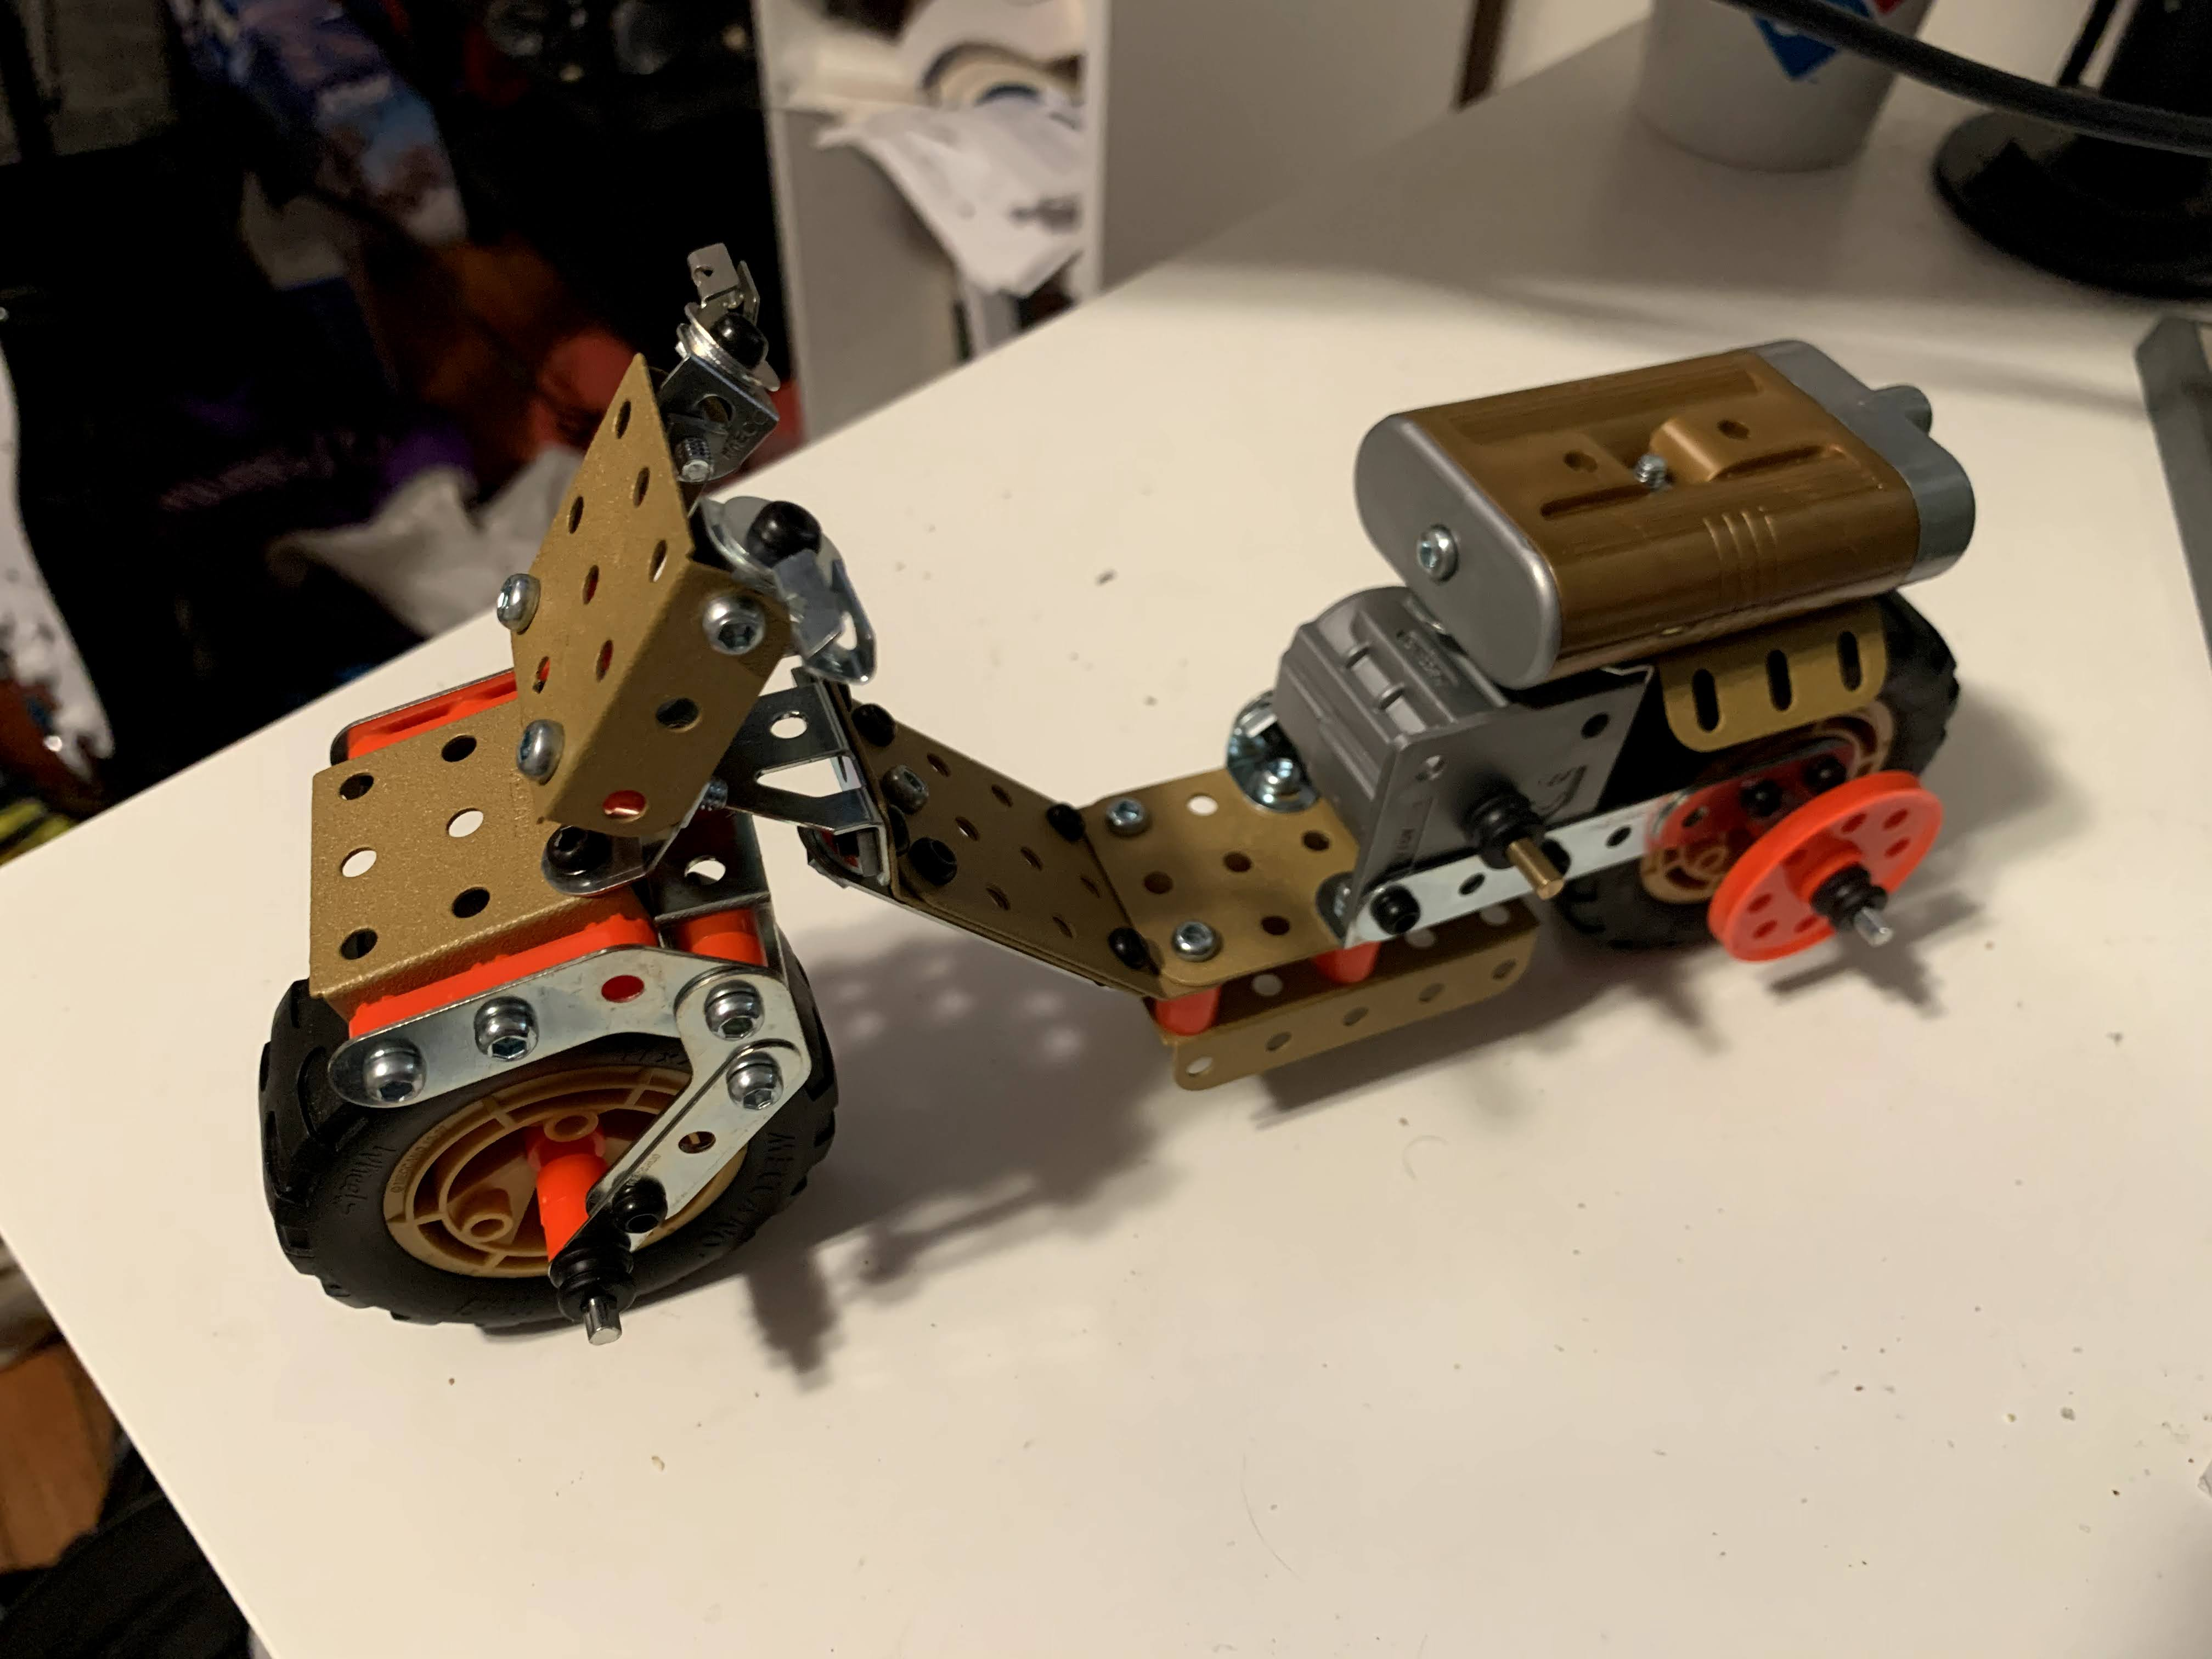
\includegraphics[width=\columnwidth]{figures/synthetic/full_bike.jpg}
  \caption{
    The fully assembled model bike.
  }\label{fig:full_bike}
\end{figure}

\subsection{Generating Data}

We found a computer-aided design (CAD) model for the Meccano kit on the
community website
GrabCAD\footnote{https://grabcad.com/library/meccano-9550-002-1}.
This CAD model appears to have been created to replicate the physical Meccano
pieces, rather than being the same model that was used to manufacture the
pieces.
In particular, we noticed a number of differences between the CAD model and the
actual Meccano parts.
We selected textures for each part of the model, trying to match the
appearance of the physical object as closely as possible.

We generated synthetic images using the Unity Perception Package~\cite{unity}.
The default setup for this package fills the background of the images that are
generated with objects that the network should learn to ignore.
Figure~\ref{fig:perception_default} shows an image generated using this default
setup.

\begin{figure}
  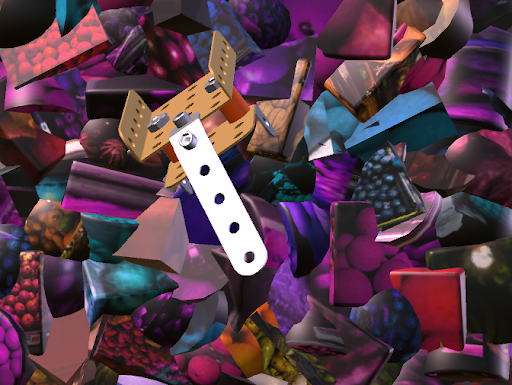
\includegraphics[width=\columnwidth]{figures/synthetic/perception_default.png}
  \caption{
    A synthetic image showing part of the bike model. The background is filled
    with distractor objects that the network should learn not to identify.
  }\label{fig:perception_default}
\end{figure}

We trained a Faster R-CNN object detector using this data.
The Unity package creates a file with bounding box and label information, and
we converted this to the format used by the TensorFlow Object Detection API.
The perception package drew bounding boxes tightly around the objects.
We added padding to these bounding boxes, to make them more like our hand-drawn
labels (which also had some padding).

Unfortunately the training process for this model did not converge.
We attempted to fix this issue by removing the background objects from the
image, and then we tried to make the objects look like they were sitting on a
wooden floor.
We accomplished this by placing the object at the bottom of the 3D scene in
Unity and texturing the floor of the scene with an image of wood from Adobe's
collection of stock images.
Figure~\ref{fig:wood_floor} shows one of these images.

\begin{figure}
  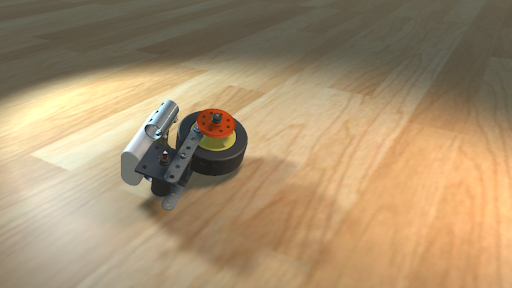
\includegraphics[width=\columnwidth]{figures/synthetic/wood_floor.png}
  \caption{
    Our first attempt at making our synthetic images look more realistic.
    This image is meant to look like an object sitting on a wood floor.
  }\label{fig:wood_floor}
\end{figure}

The Faster R-CNN model trained on this data converged; however, it performed
poorly.
One issue that we noticed was the object detector mistakenly detected lines
in the wood floor as being a model bike assembly.
Figure~\ref{fig:false_positive} shows an example of such an erroneous detection.

\begin{figure}
  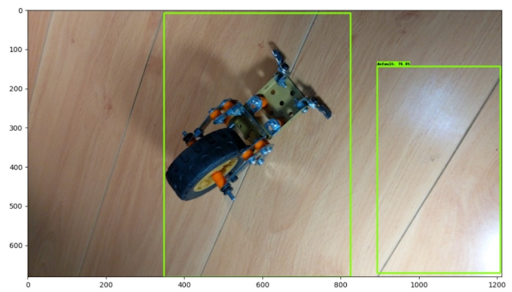
\includegraphics[width=\columnwidth]{figures/synthetic/false_positive.png}
  \caption{
    A case where our model incorrectly detected a line in the floor as an
    object of interest.
    The green bounding boxes are regions of the image that the model detected
    an object in.
  }\label{fig:false_positive}
\end{figure}

We were able to correct this issue by using additional background textures and
randomizing the lighting in the scene and the position of the camera.
We have posted our code\footnote{https://github.com/exiaohuaz/data-gen}.
Figure~\ref{fig:good_data} shows some examples of this data.

\begin{figure}
  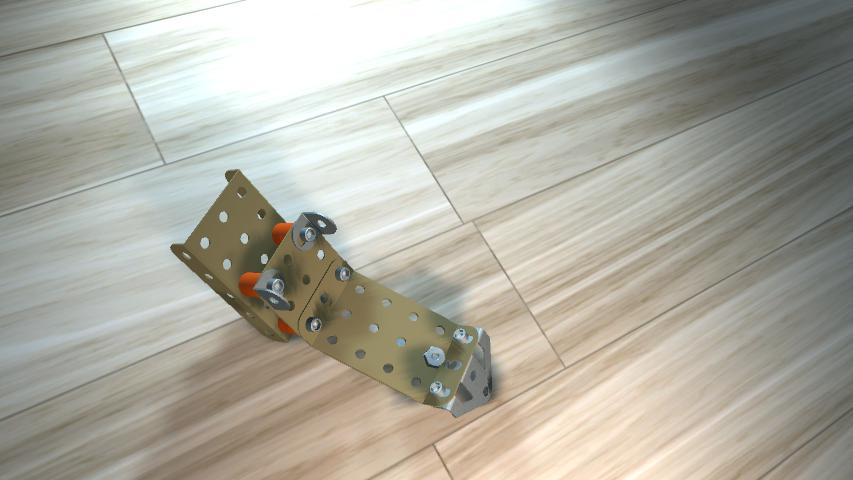
\includegraphics[width=0.5\columnwidth]{figures/synthetic/floor1.jpg}
  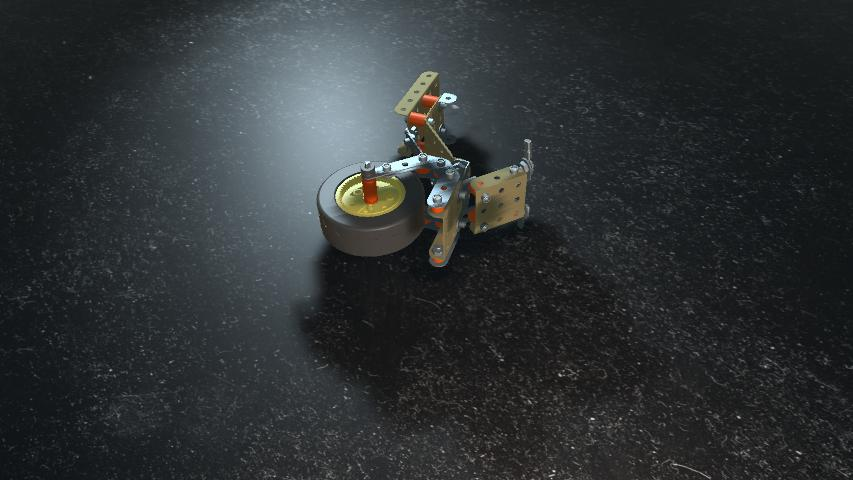
\includegraphics[width=0.5\columnwidth]{figures/synthetic/floor2.jpg}
  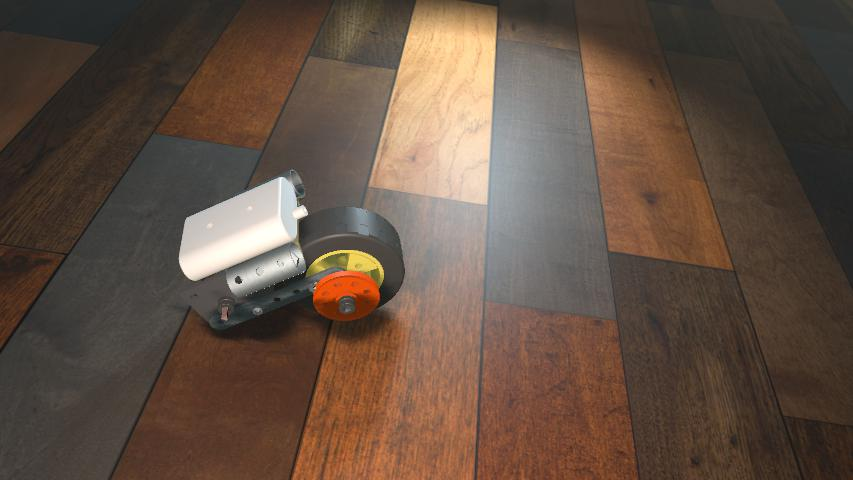
\includegraphics[width=0.5\columnwidth]{figures/synthetic/floor3.jpg}
  \caption{
    Synthetically generated images from our final set. The models trained on
    this data performed well.
  }\label{fig:good_data}
\end{figure}

After training the Faster R-CNN object detector to find the location of a
subassembly, we trained a Fast MPN-COV classifier to determine the step of the
task that is shown in the region found by the Faster R-CNN model.
Henceforth, we will use the term model pair to describe a Faster R-CNN object
detector and a Fast MPN-COV classifier created using the same training set.

\subsection{Results}

All of our training and testing data relates to
uncluttered environments with good lighting.  We assume that a human
using a WCA application can correct environmental issues to reduce
classification complexity.  For example, the user can increase the
amount of light shining on an assembly, or remove clutter from the
background.   Assuming optimal environmental conditions for a WCA assembly
task is thus reasonable.

We trained one model pair on real data that was manually labeled with
bounding boxes and class labels (15,477 images).
The remaining model pairs were trained on synthetic data sets of varying size
(12,000, 25,000, 50,000 and 75,000 images).
The labels for these images were generated by Unity.
We compared the accuracy of these model pairs.

Our test set consists of 4490 real images that are not included in any
training set.  Table~\ref{tab:meccano_accuracy} presents our results.  We
observe that the model trained on real data performs better than the
models trained on synthetic datasets with 12,000, 25,000, and 50,000
images.  However, this relationship is reversed for a model trained on
75,000 synthetic images.  Somewhere between 50,000 and 75,000 images
lies the cross-over point at which the increased number of synthetic
images more than compensates for their lower realism.

\begin{table}
  \centering
\begin{tabular}{|l||l|l|}
\hline
  Dataset Type & Training Set Size & Accuracy\\
  \hline
  \hline
  Synthetic & 12,000 & 69.6\%\\
  Synthetic & 25,000 & 79\%\\
  Synthetic & 50,000 & 84.1\%\\
  Synthetic & 75,000 & 89\%\\
  \hline
  Real & 15,477 & 84.5\%\\
\hline
\end{tabular}
  \caption{
    Classification results for our model pairs for the Meccano kit.
    Accuracy is the percentage of our 4490 test images that the pipeline of
    models classified correctly.
  }\label{tab:meccano_accuracy}
\end{table}

\section{Toy Plane}

The next kit we generated synthetic images for was a toy plane that was made up
of 3D printed plastic parts.
This kit contained six unique parts, and required four steps to assemble.
Figure~\ref{fig:assembled_plane} shows what the physical kit looks like when it
is fully assembled.
Figure~\ref{fig:plane_parts} shows the CAD models for the individual parts while
Figure~\ref{fig:plane_steps} shows the CAD models for the assembly steps.

\begin{figure}
  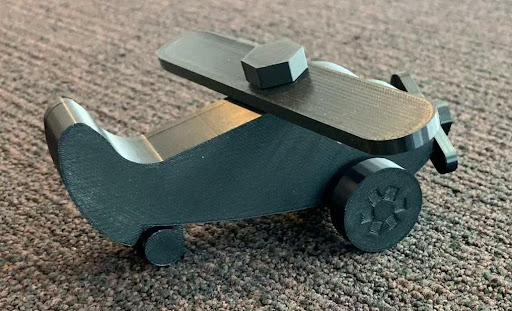
\includegraphics[width=\columnwidth]{figures/synthetic/toy_plane.jpg}
  \caption{
    The fully assembled model plane kit. All parts are 3D printed plastic.
  }\label{fig:assembled_plane}
\end{figure}

\begin{figure}
  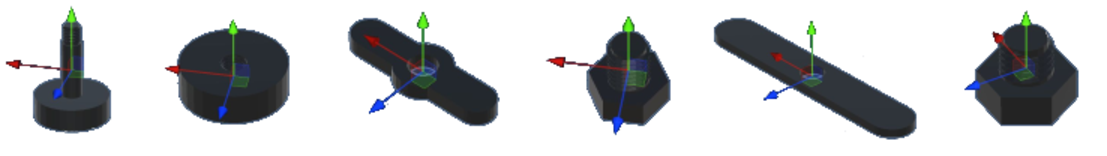
\includegraphics[width=\columnwidth]{figures/synthetic/plane_parts.pdf}
  \caption{
    CAD models for the individual model plane parts.
  }\label{fig:plane_parts}
\end{figure}

\begin{figure}
  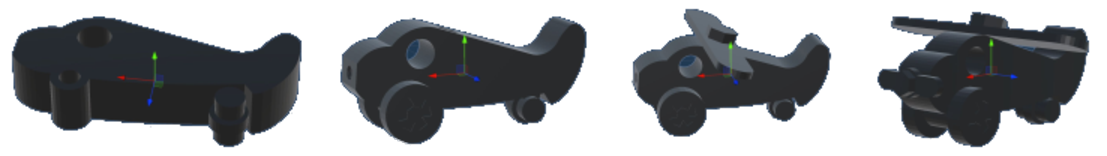
\includegraphics[width=\columnwidth]{figures/synthetic/plane_steps.pdf}
  \caption{
    CAD models for the model plane assembly steps.
  }\label{fig:plane_steps}
\end{figure}

We downloaded the CAD file for this kit from the community website
Cults~\footnote{https://cults3d.com/en/3d-model/game/toy-plane-assembled-by-bolts-and-nuts},
and then 3D printed the kit using this file.
We will refer to objects generated from a CAD model that we have access to as
being ``born digitally.''

We captured real images of the 3D printed parts using a smartphone camera,
labeled these images with CVAT, and trained a model pair on this data.
Next, we generated synthetic training images using the Unity Perception Package.
Figure~\ref{fig:plane_train} contains examples of these images.
Afterwards, we trained a model pair on these synthetic images.

Our model pairs for the toy plane were both tested on a separate set of 14,996
real images.
The results of these tests are shown in Table~\ref{tab:plane_accuracy}.
In this case, the model pair trained on 50,000 synthetic images performed better
than the model pair trained on 39,643 real images.
The model pairs for the toy plane performed worse than the model pairs for the
Meccano kit.
One possible explanation is that the fine-grained classifier for the toy plane
had 10 output labels (6 parts and 4 assembly steps), while the classifier for
the Meccano kit had 5 output labels.

\begin{figure}
  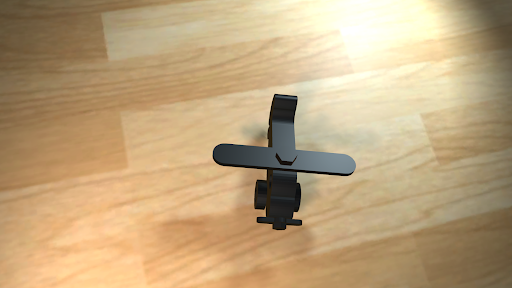
\includegraphics[width=0.5\columnwidth]{figures/synthetic/plane_train1.png}
  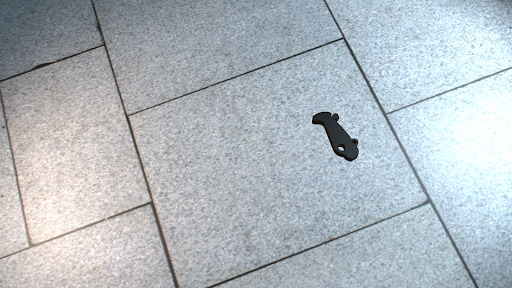
\includegraphics[width=0.5\columnwidth]{figures/synthetic/plane_train2.png}
  \caption{
    Synthetically generated training images for the toy plane kit.
  }\label{fig:plane_train}
\end{figure}

\begin{table}
  \centering
\begin{tabular}{|l||l|l|}
\hline
  Dataset Type & Training Set Size & Accuracy\\
  \hline
  \hline
  Synthetic & 50,000 & 82\%\\
  \hline
  Real & 39,643 & 76\%\\
\hline
\end{tabular}
  \caption{
    Classification results for our model pairs.
    Accuracy is the percentage of our 14,996 test images that the pipeline of
    models classified correctly.
  }\label{tab:plane_accuracy}
\end{table}

\section{Phone Sanitizer}

The final kit we generated synthetic training data for was a sanitizer for a
smartphone.
This kit contained a large metal base and several plastic parts.
Figure~\ref{} shows the kit fully assembled with all of the pieces that we had
access to.
The kit contained four unique parts, and there were five steps required to
assemble it.
Thus there were 9 output labels from the fine-grained classifier.

\begin{figure}
  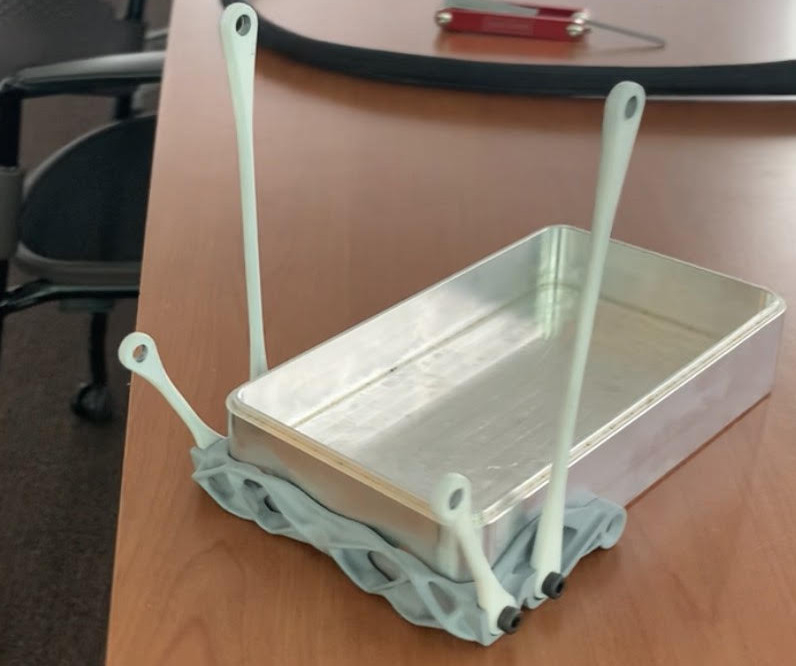
\includegraphics[width=\columnwidth]{figures/synthetic/full_sanitizer.jpg}
  \caption{
    TODO
  }\label{fig:full_sanitizer}
\end{figure}

As with the toy plane, we had access to the CAD files that the parts were
manufactured from.
We generated synthetic training images for the sanitizer using the Unity
Perception package and Autodesk A3D.
Figure~\ref{} shows images from the training set that was generated using Unity
while Figure~\ref{} shows images from the training set that was generated using
A3D.
Both sets of data were used to train model pairs that were then evaluated on
60,129 real images.
